\pdfbookmark{Общая характеристика работы}{characteristic}             % Закладка pdf
\section*{Общая характеристика работы}

\newcommand{\actuality}{\pdfbookmark[1]{Актуальность}{actuality}\underline{\textbf{\actualityTXT}}}
\newcommand{\progress}{\pdfbookmark[1]{Разработанность темы}{progress}\underline{\textbf{\progressTXT}}}
\newcommand{\aim}{\pdfbookmark[1]{Цели}{aim}\underline{{\textbf\aimTXT}}}
\newcommand{\tasks}{\pdfbookmark[1]{Задачи}{tasks}\underline{\textbf{\tasksTXT}}}
\newcommand{\aimtasks}{\pdfbookmark[1]{Цели и задачи}{aimtasks}\aimtasksTXT}
\newcommand{\novelty}{\pdfbookmark[1]{Научная новизна}{novelty}\underline{\textbf{\noveltyTXT}}}
\newcommand{\influence}{\pdfbookmark[1]{Практическая значимость}{influence}\underline{\textbf{\influenceTXT}}}
\newcommand{\methods}{\pdfbookmark[1]{Методология и методы исследования}{methods}\underline{\textbf{\methodsTXT}}}
\newcommand{\defpositions}{\pdfbookmark[1]{Положения, выносимые на защиту}{defpositions}\underline{\textbf{\defpositionsTXT}}}
\newcommand{\object}{\pdfbookmark[1]{Объект исследования}{object}\underline{\textbf{\objectTXT}}}
\newcommand{\pasport}{\pdfbookmark[1]{Соответствие диссертации паспорту научной специальности}{pasport}\underline{\textbf{\pasportTXT}}}
\newcommand{\subject}{\pdfbookmark[1]{Предмет исследования}{object}\underline{\textbf{\subjectTXT}}}
\newcommand{\reliability}{\pdfbookmark[1]{Достоверность}{reliability}\underline{\textbf{\reliabilityTXT}}}
\newcommand{\probation}{\pdfbookmark[1]{Апробация}{probation}\underline{\textbf{\probationTXT}}}
\newcommand{\contribution}{\pdfbookmark[1]{Личный вклад}{contribution}\underline{\textbf{\contributionTXT}}}
\newcommand{\publications}{\pdfbookmark[1]{Публикации}{publications}\underline{\textbf{\publicationsTXT}}}

{\actuality} 
% компоненты оптимизатора
Повышение эффективности выполнения запросов остаётся одной из центральных задач теории и практики систем управления базами данных (СУБД). Скорость выполнения запроса в базе данных в значительной степени определяется тем, насколько удачно оптимизатор выбирает план выполнения из множества допустимых альтернатив. На этот выбор влияют оценки числа строк в промежуточных результатах запроса, то есть оценки кардинальностей, стоимостная модель, которая приближённо оценивает затраты альтернативных планов, и алгоритм перебора пространства планов. Неточность хотя бы в одном из этих компонентов может приводить к выбору существенно менее эффективного плана и, как следствие, к заметному росту времени выполнения запроса \cite{10.14778/2850583.2850594}.

% тестируемся на аналитичечкой нагрузке
Особенно остро данная проблема проявляется при аналитических нагрузках. Для такого типа нагрузки характерны сложные многотабличные запросы, включающие большое число операций соединения и фильтрации, а также обработку значительных объёмов данных. Такие запросы обычно формируют широкое пространство альтернативных планов выполнения, в котором итоговая эффективность выбранного плана существенно зависит от точности оценок кардинальностей, адекватности стоимостной модели и эффективности алгоритма перебора пространства планов. Кроме того, при аналитических нагрузках влияние неточностей оптимизатора выражено особенно сильно, поскольку даже локально неудачное решение на одном из этапов плана может приводить к заметному росту общего времени выполнения запроса \cite{10.14778/2850583.2850594, 10.1145/3318464.3380584}.

Таким образом, актуальной является разработка методов повышения качества планирования запросов, которые сохраняют существующий оптимизатор СУБД, но позволяют учитывать фактические условия выполнения и направлять выбор альтернативных планов при приемлемых накладных расходах.

{\progress}
% кардинальность - развитое направление



Одним из наиболее подробно исследованных направлений в области интеллектуальной оптимизации запросов являются методы повышения точности оценок кардинальностей \cite{10.14778/3485450.3485459, 10.1145/3514221.3526154}. Для этой задачи предложен широкий спектр подходов~--- от классических статистических методов \cite{10.1145/376284.375686} до современных обучаемых моделей \cite{kipf2018learnedcardinalitiesestimatingcorrelated}. В то же время даже существенное повышение точности оценок кардинальностей не устраняет полностью проблему выбора неоптимального плана, поскольку на итоговое качество оптимизации влияют также стоимостная модель и ограничения алгоритма перебора пространства планов \cite{10.14778/2850583.2850594, 10.14778/1687627.1687739}. Вопросы оценки кардинальностей исследуются в работах N.~Bruno, S.~Chaudhuri, L.~Gravano, A.~Kipf, J.~Sun, K.~Kim и других авторов \cite{10.1145/376284.375686,kipf2018learnedcardinalitiesestimatingcorrelated,10.14778/3485450.3485459,10.1145/3514221.3526154}.

% интеграция с существующим оптимизатором
При этом полная замена штатного оптимизатора внешней моделью в практических СУБД связана с высокой инженерной сложностью и не всегда целесообразна. Современный оптимизатор содержит большое число правил преобразования запросов, эвристик, механизмов учёта физических операторов, индексов, статистики и параметров среды выполнения. Его замена требует воспроизведения значительной части этой функциональности, а также обеспечения корректности, устойчивости и переносимости решений при изменении данных, схемы, рабочей нагрузки и конфигурации системы. Поэтому практически значимым направлением являются гибридные методы, которые сохраняют существующий оптимизатор, но улучшают отдельные компоненты процесса планирования или направляют выбор альтернативных планов через предусмотренные СУБД механизмы управления \cite{zhu2023lero, anneser2023autosteer}.

% стоимостная модель



Одной из таких точек интеграции является стоимостная модель оптимизатора. Существующие исследования показывают, что повышение точности стоимостной модели может улучшать качество выбора плана оптимизатором. На практике это достигается как за счёт калибровки параметров стоимостной модели, так и за счёт обучаемых моделей оценки планов, интегрируемых в оптимизатор \cite{Lan_2021}. Однако такие решения обычно требуют накопления обучающих данных, регулярного переобучения при изменении нагрузки и нередко плохо переносятся между различными конфигурациями систем. Кроме того, ручная настройка параметров стоимости требует высокой квалификации администратора базы данных, а калибровка на специально сформированной синтетической нагрузке не всегда отражает реальные условия эксплуатации. Поэтому актуальной остаётся задача адаптивной настройки параметров стоимостной модели по телеметрии фактически выполняемых запросов, без запуска отдельной калибровочной нагрузки, без обучения отдельной модели \cite{10.1145/3514221.3526154, 10.1145/3318464.3380584}. Вопросам построения и настройки стоимостных моделей посвящены работы T.~Siddiqui и других исследователей; состояние данного направления обобщено H.~Lan, Z.~Bao и Y.~Peng \cite{10.1145/3318464.3380584,Lan_2021}.

% перебор пространства планов
Наряду с оценками кардинальностей и стоимостной моделью существенное влияние на итоговое качество оптимизации оказывает алгоритм перебора пространства планов. Из-за высокой вычислительной сложности полного перебора оптимизаторы используют различные ограничения и эвристики, позволяющие удерживать время планирования в разумных пределах, но способные приводить к пропуску части потенциально эффективных альтернатив \cite{Lan_2021}. Поэтому отдельный практический интерес представляют методы, позволяющие направлять выбор планов без полной замены существующего оптимизатора.

% подсказки оптимизатору



Одним из практических средств направленного воздействия на поведение оптимизатора являются подсказки, позволяющие задавать дополнительные ограничения или предпочтения при построении плана выполнения и тем самым влиять на множество рассматриваемых альтернатив и итоговый план выполнения. В последние годы активно развиваются подходы, основанные на машинном обучении, в которых механизм выбора подсказок используется для управления существующим оптимизатором без его полной замены. Вместе с тем автоматический подбор подсказок остаётся сложной задачей: пространство возможных конфигураций может быть достаточно большим, полный перебор требует значительных затрат, ошибочная подсказка способна ухудшить план, а обучаемые решения часто требуют предварительного накопления данных и дополнительного сопровождения \cite{10.1145/3448016.3452838, zhu2023lero}. Методы обучаемого выбора планов и управления штатным оптимизатором посредством подсказок развиваются, в частности, в работах R.~Marcus, R.~Zhu, C.~Anneser и их соавторов \cite{10.1145/3448016.3452838,zhu2023lero,anneser2023autosteer}.

% режимы автоматического подбора подсказок
В задачах автоматического подбора подсказок можно выделить два практически различных режима, различающихся допустимыми накладными расходами и целью оптимизации. Первый режим связан с онлайн-оптимизацией, когда рекомендация должна быть получена непосредственно перед выполнением запроса, а время выбора подсказки должно быть существенно меньше ожидаемого выигрыша от её применения. Такой сценарий характерен для потоков аналитических запросов, где требуется быстро принять решение для нового запроса на основе уже накопленного опыта, не выполняя дорогостоящий перебор и не запуская дополнительное обучение на целевой нагрузке. 

Второй режим связан с офлайн-оптимизацией или предварительной настройкой, когда для запроса или группы похожих запросов допустимо выделить ограниченный бюджет пробных запусков. Такой сценарий оправдан, например, для часто повторяющихся аналитических запросов, ускорение которых будет использоваться многократно. В этом случае основная цель состоит не в мгновенной рекомендации, а в нахождении более эффективной конфигурации подсказок оптимизатору. Поэтому онлайн- и офлайн-постановки соответствуют разным практическим задачам: первая ориентирована на минимальные накладные расходы при принятии решения, вторая~--- на более тщательный поиск качественного решения при заранее заданном бюджете оптимизации.

% языковые модели для БД
%Дополнительный интерес связан с быстрым развитием больших языковых моделей. В настоящее время большие языковые модели в области баз данных применяются по нескольким крупным направлениям. Во-первых, они используются для построения интерфейсов на естественном языке к данным, включая преобразование запросов на естественном языке в SQL и поддержку диалогового взаимодействия с базой данных \cite{Zhou2024DBGPTLL,10.1007/s11704-025-50592-w}. Во-вторых, они применяются для обработки структурированных представлений базы данных, включая анализ таблиц, схем таблиц и связанных с ними метаданных, а также для сопоставления схем и интеграции источников данных \cite{10.1007/s11704-024-40763-6,parciak2024schemamatchinglargelanguage}. В-третьих, языковые модели используются для задач сопровождения и настройки СУБД, включая интеллектуальные средства работы с документацией \cite{Zhou2024DBGPTLL,10.1007/s00778-023-00831-y}. В-четвёртых, активно исследуется применение больших языковых моделей для оптимизации запросов, включая переписывание запросов, а в отдельных работах - и непосредственное построение планов выполнения \cite{li2024llmr2,song2026quitequeryrewriterules,10.1145/3626246.3654732}. Вместе с тем существующие подходы на основе больших языковых моделей имеют ряд ограничений. К их числу относятся зависимость качества результата от выбора подсказок и примеров, слабый учёт физических характеристик СУБД и данных, трудности обеспечения эквивалентности преобразований и повышенные риски галлюцинаций. Дополнительно в обзорах отмечаются сохраняющиеся проблемы обработки сложных запросов, устойчивости, безопасности и вычислительной стоимости таких систем \cite{Zhou2024DBGPTLL, song2026quitequeryrewriterules, 10.1007/s11704-025-50592-w}.

% языковые модели для БД



Дополнительный интерес к указанным задачам связан с быстрым развитием больших языковых моделей и расширением области их применения в СУБД. В настоящее время такие модели исследуются для построения интерфейсов на естественном языке к данным, обработки таблиц, схем и метаданных, сопровождения и настройки СУБД, а также для задач оптимизации запросов, включая переписывание запросов и построение вариантов планов выполнения \cite{Zhou2024DBGPTLL,10.1007/s11704-025-50592-w,10.1007/s11704-024-40763-6,parciak2024schemamatchinglargelanguage,10.1007/s00778-023-00831-y,li2024llmr2,song2026quitequeryrewriterules,10.1145/3626246.3654732}. Это показывает, что большие языковые модели становятся одним из перспективных инструментов для задач, связанных с анализом, настройкой и автоматизацией работы СУБД. Поэтому актуальным является исследование способов их использования не только в пользовательских интерфейсах или генерации SQL-запросов, но и в задачах повышения качества планирования запросов. Применение больших языковых моделей к задачам сопровождения СУБД, переписывания запросов и построения планов рассматривается в работах I.~Trummer, Z.~Li, Y.~Song, M.~Urban, C.~Binnig и других авторов \cite{10.1007/s00778-023-00831-y,li2024llmr2,song2026quitequeryrewriterules,10.1145/3626246.3654732}.

% режимы использования языковых моделей
При этом способ применения больших языковых моделей должен соответствовать ограничениям конкретной постановки оптимизации. В режиме онлайн-рекомендации основным ограничением является время принятия решения: подсказку необходимо выбрать до выполнения запроса, а накладные расходы на оптимизацию должны быть малы. Поэтому в такой постановке целесообразно использовать языковую модель в облегчённом режиме, извлекая из неё компактное представление, пригодное для быстрого сопоставления нового запроса с ранее накопленным опытом. В режиме офлайн-оптимизации или предварительной настройки, напротив, допустим ограниченный бюджет пробных запусков, а основной целью является получение наиболее эффективной найденной конфигурации подсказок оптимизатору. В этом случае языковая модель может использоваться более полно, как компонент, принимающий решения в итеративном процессе оптимизации.

% актуальность исследования
%Таким образом, анализ степени разработанности темы показывает, что к настоящему времени наиболее подробно исследованы методы оценки кардинальностей и отдельные подходы, основанные на обучении, для выбора планов и подсказок. Вместе с тем в меньшей степени разработаны подходы, связанные с онлайн-настройкой стоимостной модели по телеметрии реальных запросов без обучения отдельной модели. Существенный интерес также представляют быстрые методы рекомендации подсказок, использующие  большие языковые модели, но не требующие длительной генерации и специального обучения. При этом применение больших языковых моделей в задачах оптимизации и сопровождения баз данных всё ещё связано с рядом открытых вопросов. К ним относятся учёт физических характеристик конкретной СУБД и статистики данных, проверка корректности предлагаемых решений, снижение задержек инференса и стоимости дообучения, а также переносимость методов между различными схемами данных, рабочими нагрузками и конфигурациями вычислительной среды.

% актуальность исследования

Таким образом, анализ степени разработанности темы показывает, что к настоящему времени наиболее подробно исследованы методы оценки кардинальностей и отдельные обучаемые подходы к оценке и выбору планов. Вместе с тем остаются открытыми вопросы настройки стоимостной модели по телеметрии реальных запросов без отдельной обучаемой модели. Существенный интерес также представляют методы рекомендации подсказок, использующие возможности больших языковых моделей без необходимости длительной генерации при обработке каждого запроса. Применение больших языковых моделей в задачах оптимизации и сопровождения баз данных всё ещё связано с рядом открытых вопросов, включая учёт физических характеристик конкретной СУБД и статистики данных, проверку корректности предлагаемых решений, снижение задержек инференса и стоимости дообучения, а также переносимость методов между различными схемами данных, рабочими нагрузками и конфигурациями вычислительной среды.


{\object} Планирование запросов в реляционных системах управления базами данных.

{\subject} Методы повышения качества планирования запросов в реляционных системах управления базами данных.

{\aim} данной работы является разработка и экспериментальное обоснование комплекса методов повышения качества планирования запросов в реляционных системах управления базами данных, включающего адаптивную настройку параметров стоимостной модели, рекомендацию подсказок оптимизатору на основе векторных представлений планов выполнения, формируемых большой языковой моделью, и агентный итеративный поиск подсказок.

Для~достижения поставленной цели необходимо решить следующие {\tasks}:
\begin{enumerate}[beginpenalty=10000] % https://tex.stackexchange.com/a/476052/104425
  \item Провести анализ современного состояния методов оптимизации запросов в реляционных СУБД и определить ограничения существующих подходов, связанные с настройкой стоимостной модели, управлением выбором альтернативных планов и применением обучаемых методов в составе существующего оптимизатора.
  \item Разработать метод адаптивной настройки параметров стоимостной модели, обеспечивающий адаптацию к фактическим условиям выполнения запросов по телеметрии эксплуатационной нагрузки, без запуска отдельной калибровочной нагрузки и без обучения отдельной модели. Оценить влияние метода на согласованность между оценочной стоимостью и фактическим временем выполнения.
  \item Разработать метод рекомендации подсказок оптимизатору для онлайн-сценария, в котором выбор управляющего воздействия должен выполняться с малыми накладными расходами на основе ранее накопленного опыта, без обучения на целевой рабочей нагрузке. Исследовать возможность использования векторных представлений, формируемых большой языковой моделью, для сопоставления планов выполнения и использования ранее найденных подсказок для новых запросов.
  \item  Разработать метод итеративного поиска подсказок оптимизатору для офлайн-сценария или предварительной настройки, в котором допустим ограниченный бюджет пробных запусков, а выбор очередного действия выполняется с учётом текущего состояния поиска. Исследовать эффективность применения большой языковой модели в качестве компонента принятия решений в таком контуре.
  \item Провести экспериментальную оценку разработанных методов на репрезентативных аналитических наборах запросов и сравнить их с соответствующими базовыми и альтернативными подходами по времени выполнения, качеству выбора планов и стоимости оптимизации.
\end{enumerate}

{\novelty}
\begin{enumerate}[beginpenalty=10000] % https://tex.stackexchange.com/a/476052/104425
\item Разработан метод адаптивной настройки параметров стоимостной модели оптимизатора, отличающийся использованием агрегированной модели состояния буферного кэша на уровне отношений и настройкой параметров по телеметрии фактически выполняемых запросов. Метод позволяет уточнять параметры ввода-вывода и вычислительной составляющей стоимости без отдельной калибровочной нагрузки и без замены штатного оптимизатора.

\item Разработан метод рекомендации подсказок оптимизатору на основе сопоставления планов выполнения в пространстве векторных представлений. В методе предобученная языковая модель используется для формирования векторных представлений планов выполнения, а выбор кандидата выполняется на основе сопоставления этих представлений, после чего выполняется дополнительная проверка согласованности. Метод позволяет использовать ранее накопленный опыт выполнения запросов без дообучения модели на целевой рабочей нагрузке.

\item Разработан агентный метод итеративного поиска подсказок оптимизатору в замкнутом контуре обратной связи с системой управления базами данных. Метод  основан на использовании большой языковой модели для пошагового выбора действий и повышает результативность поиска эффективных конфигураций подсказок при ограниченном бюджете пробных запусков.
\end{enumerate}

{\methods} В диссертационной работе для решения поставленных задач использовались методы теории баз данных, методы машинного обучения, методы математической статистики, методы математического и компьютерного моделирования, методы регрессионного анализа, методы анализа данных, а также методы вычислительного эксперимента. Экспериментальные исследования выполнялись на аналитических наборах запросов с применением сравнительного анализа времени выполнения, корреляционных характеристик стоимостной модели и показателей качества выбора планов выполнения.

{\theoreticalSignificance} Предложен и обоснован комплекс методов повышения качества планирования SQL-запросов в реляционных СУБД на основе адаптации стоимостной модели, сопоставления планов выполнения в пространстве векторных представлений и итеративного поиска подсказок оптимизатору. Данный подход развивает методы гибридной оптимизации запросов, в которых средства машинного обучения дополняют штатный оптимизатор без его полной замены.

{\influence} заключается в том, что предложенные методы могут быть использованы для повышения качества выбора планов выполнения в СУБД в рамках существующего оптимизатора. Разработанные решения ориентированы на применение в аналитических нагрузках, допускают внедрение с ограниченными изменениями в системе и позволяют уменьшить объём ручной настройки параметров и перебора конфигураций подсказок. Практическая значимость исследования подтверждается актом о внедрении результатов работы.

{\defpositions}
\begin{enumerate}[beginpenalty=10000] % https://tex.stackexchange.com/a/476052/104425
\item Метод адаптивной настройки параметров стоимостной модели оптимизатора по телеметрии фактически выполняемых запросов, учитывающий состояние буферного кэша, позволяет повышать согласованность между стоимостью плана и фактическим временем его выполнения, а также улучшать качество выбора плана без отдельного этапа калибровки.

\item Метод рекомендации подсказок оптимизатору на основе сопоставления планов выполнения, использующий векторные представления планов, формируемые большой языковой моделью, позволяет использовать ранее накопленный опыт для выбора эффективных конфигураций подсказок без обучения на целевой рабочей нагрузке.

\item Агентный метод итеративного поиска подсказок оптимизатору на основе большой языковой модели позволяет направленно искать эффективные конфигурации подсказок в замкнутом контуре обратной связи с системой управления базами данных и повышать качество оптимизации при ограниченном бюджете пробных запусков по сравнению с базовыми и альтернативными методами.
\end{enumerate}

{\pasport} Тема диссертационного исследования и его содержание соответствуют требованиям паспорта специальности ВАК 2.3.5 – Математическое и программное обеспечение вычислительных систем, комплексов и компьютерных сетей:
\begin{enumerate}
    \setcounter{enumi}{2}
    \item Модели, методы, архитектуры, алгоритмы, языки и программные инструменты организации взаимодействия программ и программных систем.
    \item Интеллектуальные системы машинного обучения, управления базами данных и знаний, инструментальные средства разработки цифровых продуктов. 
\end{enumerate}

{\reliability} полученных результатов обеспечивается использованием стандартных и широко применяемых в исследовательской практике бенчмарков для оценки методов оптимизации запросов, сопоставлением предложенных методов с базовыми и альтернативными подходами, проведением экспериментов в контролируемых условиях, а также использованием воспроизводимой методики оценки, включающей повторные измерения и анализ совокупных показателей времени выполнения и качества принимаемых решений.

{\probation}
Основные результаты работы докладывались на:
\begin{enumerate}
    \item семинар Московской секции ACM SIGMOD в 2026 году, семинар лаборатории информационных систем ИСИ СО РАН в 2025 году, семинар русскоязычного сообщества AGI в 2025 году;
    \item Международная конференция <<Знания -- Онтологии -- Теории>> (ЗОНТ), 2025;
    \item IEEE XVII International Conference on Actual Problems of Electronic Instrument Engineering (APEIE), 2025.
\end{enumerate}
%Основные результаты работы докладывались на:
%перечисление основных конференций, симпозиумов и~т.\:п.

{\contribution} Работа выполнена в составе научной группы. Исходные идеи и постановки задач, рассматриваемых в главах 2–4 диссертации, развивались в неразрывном сотрудничестве с соавторами. Автором лично выполнены программная реализация предложенных методов, подготовка данных, планирование и проведение вычислительных экспериментов, обработка и анализ полученных результатов, а также подготовка текста диссертации. В главе 2 автором самостоятельно разработана агрегированная модель состояния буферного кэша, выполнены программная реализация метода адаптивной настройки параметров стоимостной модели, проведение экспериментальных исследований и анализ результатов; формализация части метода, связанной с настройкой параметров процессора, выполнена совместно с научным руководителем. В главе 3 автором самостоятельно разработаны предсказательная модель и метод рекомендации подсказок оптимизатору на основе сопоставления планов выполнения, выполнены их реализация, подготовка экспериментальных данных, проведение экспериментов и анализ результатов. В главе 4 разработка агентного метода итеративного поиска подсказок оптимизатору, формирование контекста и диалогового набора данных, реализация агентов, проведение экспериментов и анализ результатов выполнены автором самостоятельно.

\ifnumequal{\value{bibliosel}}{1}
{%%% Встроенная реализация с загрузкой файла через движок bibtex8. (При желании, внутри можно использовать обычные ссылки, наподобие `\cite{vakbib1,vakbib2}`).
    \nocite{vasilenko2024acm}
    \nocite{vasilenko2026plan_mapping}
    \nocite{vasilenko_article_inpress}
    \nocite{11289347}
    \nocite{vasilenko2025}
    \nocite{burl2025}
    \nocite{vasilenko_patent}
    {\publications} Основные результаты диссертационного исследования отражены в 6 научных публикациях, включая 2 статьи в журналах, индексируемых в международной базе данных Scopus, из которых 1 статья опубликована в журнале первого квартиля и 1 статья~--- в журнале второго квартиля по SCImago Journal Rank; 1 статью в журнале, рекомендованном ВАК; а также 3 работы, опубликованные в сборниках и трудах международных и всероссийских научных конференций, из которых 1 работа индексируется в базе данных Scopus. Получены свидетельство о государственной регистрации программы для ЭВМ и акт о внедрении результатов исследования.
}%
{%%% Реализация пакетом biblatex через движок biber
    \begin{refsection}[bl-author, bl-registered]
        % Это refsection=1.
        % Процитированные здесь работы:
        %  * подсчитываются, для автоматического составления фразы "Основные результаты ..."
        %  * попадают в авторскую библиографию, при usefootcite==0 и стиле `\insertbiblioauthor` или `\insertbiblioauthorgrouped`
        %  * нумеруются там в зависимости от порядка команд `\printbibliography` в этом разделе.
        %  * при использовании `\insertbiblioauthorgrouped`, порядок команд `\printbibliography` в нём должен быть тем же (см. biblio/biblatex.tex)
        %
        % Невидимый библиографический список для подсчёта количества публикаций:
        \phantom{\printbibliography[heading=nobibheading, section=1, env=countauthorvak,          keyword=biblioauthorvak]%
        \printbibliography[heading=nobibheading, section=1, env=countauthorwos,          keyword=biblioauthorwos]%
        \printbibliography[heading=nobibheading, section=1, env=countauthorscopus,       keyword=biblioauthorscopus]%
        \printbibliography[heading=nobibheading, section=1, env=countauthorconf,         keyword=biblioauthorconf]%
        \printbibliography[heading=nobibheading, section=1, env=countauthorother,        keyword=biblioauthorother]%
        \printbibliography[heading=nobibheading, section=1, env=countregistered,         keyword=biblioregistered]%
        \printbibliography[heading=nobibheading, section=1, env=countauthorpatent,       keyword=biblioauthorpatent]%
        \printbibliography[heading=nobibheading, section=1, env=countauthorprogram,      keyword=biblioauthorprogram]%
        \printbibliography[heading=nobibheading, section=1, env=countauthor,             keyword=biblioauthor]%
        \printbibliography[heading=nobibheading, section=1, env=countauthorvakscopuswos, filter=vakscopuswos]%
        \printbibliography[heading=nobibheading, section=1, env=countauthorscopuswos,    filter=scopuswos]}%
        %
        \nocite{*}%
        %
        {\publications} Основные результаты по теме диссертации изложены в~\arabic{citeauthor}~печатных изданиях,
        \arabic{citeauthorvak} из которых изданы в журналах, рекомендованных ВАК%
        \ifnum \value{citeauthorscopuswos}>0%
            , \arabic{citeauthorscopuswos} "--- в~периодических научных журналах, индексируемых Web of~Science и Scopus%
        \fi%
        \ifnum \value{citeauthorconf}>0%
            , \arabic{citeauthorconf} "--- в~тезисах докладов.
        \else%
            .
        \fi%
        \ifnum \value{citeregistered}=1%
            \ifnum \value{citeauthorpatent}=1%
                Зарегистрирован \arabic{citeauthorpatent} патент.
            \fi%
            \ifnum \value{citeauthorprogram}=1%
                Зарегистрирована \arabic{citeauthorprogram} программа для ЭВМ.
            \fi%
        \fi%
        \ifnum \value{citeregistered}>1%
            Зарегистрированы\ %
            \ifnum \value{citeauthorpatent}>0%
            \formbytotal{citeauthorpatent}{патент}{}{а}{}%
            \ifnum \value{citeauthorprogram}=0 . \else \ и~\fi%
            \fi%
            \ifnum \value{citeauthorprogram}>0%
            \formbytotal{citeauthorprogram}{программ}{а}{ы}{} для ЭВМ.
            \fi%
        \fi%
        % К публикациям, в которых излагаются основные научные результаты диссертации на соискание учёной
        % степени, в рецензируемых изданиях приравниваются патенты на изобретения, патенты (свидетельства) на
        % полезную модель, патенты на промышленный образец, патенты на селекционные достижения, свидетельства
        % на программу для электронных вычислительных машин, базу данных, топологию интегральных микросхем,
        % зарегистрированные в установленном порядке.(в ред. Постановления Правительства РФ от 21.04.2016 N 335)
    \end{refsection}%
    \begin{refsection}[bl-author, bl-registered]
        % Это refsection=2.
        % Процитированные здесь работы:
        %  * попадают в авторскую библиографию, при usefootcite==0 и стиле `\insertbiblioauthorimportant`.
        %  * ни на что не влияют в противном случае

        %\nocite{progbib1}%program
        %\nocite{bib1}%other
        %\nocite{confbib1}%conf
    \end{refsection}%
        %
        % Всё, что вне этих двух refsection, это refsection=0,
        %  * для диссертации - это нормальные ссылки, попадающие в обычную библиографию
        %  * для автореферата:
        %     * при usefootcite==0, ссылка корректно сработает только для источника из `external.bib`. Для своих работ --- напечатает "[0]" (и даже Warning не вылезет).
        %     * при usefootcite==1, ссылка сработает нормально. В авторской библиографии будут только процитированные в refsection=0 работы.
}


 % Характеристика работы по структуре во введении и в автореферате не отличается (ГОСТ Р 7.0.11, пункты 5.3.1 и 9.2.1), потому её загружаем из одного и того же внешнего файла, предварительно задав форму выделения некоторым параметрам

%Диссертационная работа была выполнена при поддержке грантов \dots

%\underline{\textbf{Объем и структура работы.}} Диссертация состоит из~введения,
%четырех глав, заключения и~приложения. Полный объем диссертации
%\textbf{ХХХ}~страниц текста с~\textbf{ХХ}~рисунками и~5~таблицами. Список
%литературы содержит \textbf{ХХX}~наименование.

\underline{\textbf{Объем и структура работы.}} Диссертация состоит из введения, 4 глав, заключения и 3 приложений. Полный объём диссертации составляет 146 страниц, включая 29 рисунков и 14 таблиц. Список литературы содержит 70 наименований.

\pdfbookmark{Содержание работы}{description}                          % Закладка pdf
\section*{Содержание работы}
Во \underline{\textbf{введении}} обосновывается актуальность исследований, проводимых в~рамках данной диссертационной работы, приводится обзор научной литературы по~изучаемой проблеме, формулируется цель, ставятся задачи работы, излагается научная новизна и практическая значимость представляемой работы. 


\underline{\textbf{Первая глава}} посвящена обзору развития методов планирования SQL-запросов - от классических стоимостных оптимизаторов до современных обучаемых и гибридных подходов. Показано, что качество выбора плана определяется тремя основными компонентами: точностью оценок кардинальностей, качеством стоимостной модели и эффективностью перебора пространства альтернативных планов. При этом традиционные оптимизаторы сохраняют ряд фундаментальных ограничений: ошибки в оценке кардинальностей, приближённый характер стоимостной модели, необходимость жёстких эвристик при переборе и слабую адаптацию к изменяющейся среде выполнения.

Далее в главе рассматриваются основные направления современных исследований: обучаемые методы оценки кардинальностей, обучаемые стоимостные модели, методы выбора плана и подбора подсказок, а также генеративные подходы и большие языковые модели. На основе обзора делается вывод, что наиболее практичными являются не попытки полной замены оптимизатора, а гибридные методы, совместимые с существующей архитектурой СУБД и улучшающие отдельные компоненты процесса планирования. В связи с этим в диссертации выделяются три основных направления: адаптивная настройка параметров стоимостной модели, рекомендация подсказок оптимизатору на основе сопоставления планов выполнения и агентный метод итеративного поиска подсказок при ограниченном бюджете пробных запусков.

Отдельно обосновывается выбор экспериментальной базы. Для исследования используются аналитические бенчмарки TPC-H, JOB и CEB, поскольку именно в аналитических нагрузках ошибки оптимизатора наиболее сильно влияют на итоговое время выполнения. Таким образом, глава формирует теоретическую и методическую основу для последующих глав диссертации, в которых последовательно рассматриваются три предложенных направления улучшения планирования запросов.

Во \underline{\textbf{второй главе}} рассматривается задача повышения качества работы оптимизатора запросов за счёт адаптивной настройки параметров стоимостной модели по телеметрии фактически выполняемых запросов. Предложенный метод, в отличие от существующих подходов, основанных на выполнении специальной калибровочной нагрузки, не требует запуска дополнительных калибровочных запросов и использует информацию, формируемую в процессе эксплуатации системы.

В стоимостных оптимизаторах план выполнения выбирается на основе оценочной стоимости, которая вычисляется как сумма стоимостей отдельных операторов плана. Стоимость оператора задаётся через параметры стоимостной модели и оценки объёмов работы: числа обрабатываемых кортежей, операций, индексных записей и прочитанных страниц. В PostgreSQL и openGauss к основным параметрам относятся три параметра вычислительной составляющей: \(cpu\_tuple\_cost\), \(cpu\_index\_tuple\_cost\), \(cpu\_operator\_cost\), а также два параметра ввода-вывода: \(seq\_page\_cost\) и \(random\_page\_cost\). В общем виде стоимость оператора может быть записана как
\[
Cost_{operator}=c_t n_t+c_o n_o+c_s n_s+c_i n_i+c_r n_r,
\]
где коэффициенты \(c_t, c_o, c_s, c_i, c_r\) соответствуют параметрам стоимостной модели, а величины \(n_t, n_o, n_s, n_i, n_r\) характеризуют оцениваемый объём выполняемой работы. Следовательно, неточная настройка этих параметров приводит к несогласованности между оценочной стоимостью и фактическим временем выполнения и может вести к выбору неэффективного плана.

Предложенный метод включает два взаимосвязанных компонента. Первый компонент предназначен для уточнения параметров ввода-вывода стоимостной модели и основан на оценке состояния буферного кэша на уровне отношений. Стандартная стоимостная модель различает последовательный и непоследовательный доступ к страницам с помощью параметров \(seq\_page\_cost\) и \(random\_page\_cost\). Однако фактическая стоимость непоследовательного доступа существенно зависит от того, находится ли требуемая страница в буферном кэше или должна быть прочитана с диска. На этапе планирования СУБД обычно не располагает точной информацией о текущей доле страниц каждого отношения в буфере, а прямое отслеживание состояния отдельных страниц создаёт дополнительные накладные расходы.

Поэтому в работе предлагается не восстанавливать точный состав буферного кэша, а моделировать его состояние агрегированно, на уровне отношений. Основная идея состоит в том, что каждое выполнение запроса даёт два наблюдаемых сигнала: число обращений к страницам, обслуженных из памяти, и число страниц, прочитанных с диска. Первый сигнал указывает на повторное использование уже находящихся в буфере страниц и повышает их устойчивость к вытеснению. Второй сигнал означает загрузку новых страниц и создаёт давление на ограниченный буферный кэш.

Для приближённого учёта этих эффектов для каждого отношения \(T\) вводится распределение \(c_T[u]\) по бинам защищённости \(u=0,\ldots,U\). Значение \(c_T[u]\) показывает, сколько страниц отношения находится в буфере и имеет уровень защищённости \(u\). Страницы в бинах с большим \(u\) считаются более часто используемыми и вытесняются позже, а страницы в бине \(u=0\) рассматриваются как первые кандидаты на вытеснение. Схема изменения такого распределения при обращениях к буферному кэшу показана на рисунке~\ref{fig:usage-bins}.

\begin{figure}[h]
  \centering
   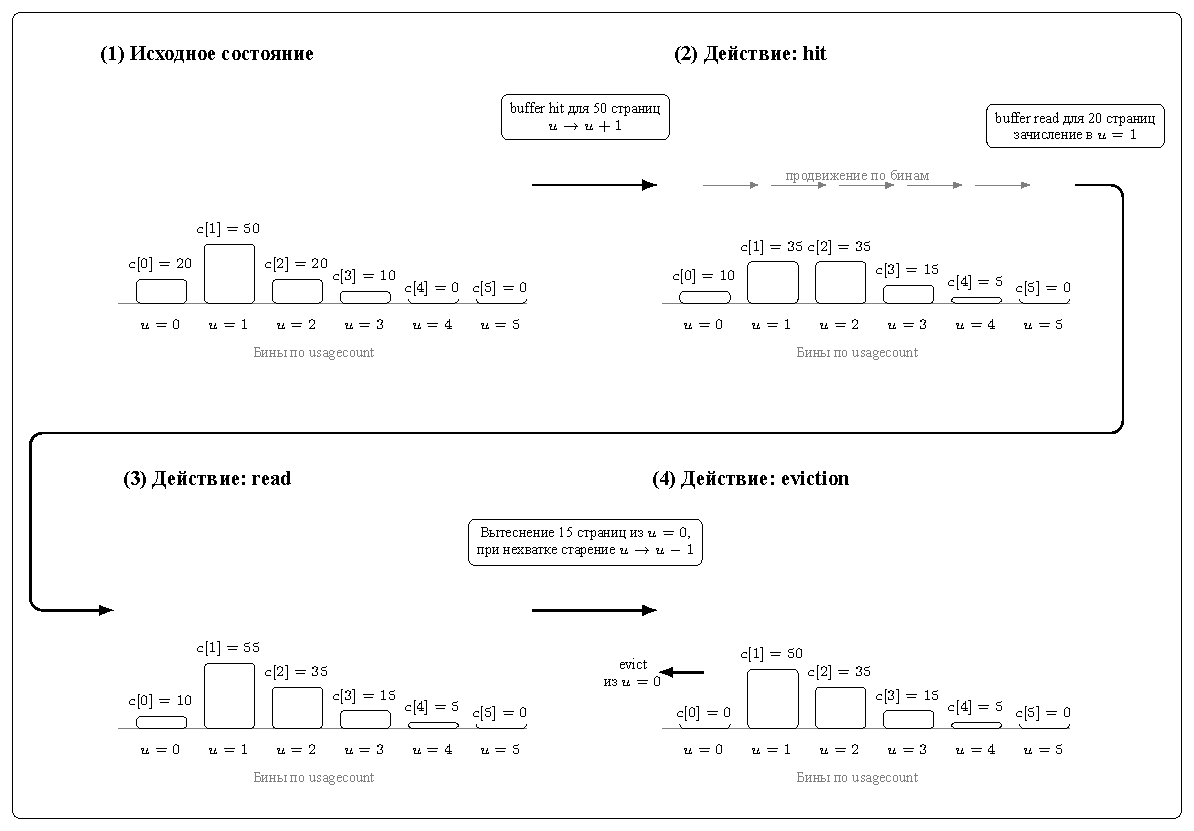
\includegraphics[width=0.85\linewidth]{images/acm_bins.pdf}
  \caption{Агрегированная модель распределения страниц по бинам защищённости и изменение этого распределения при обращениях к буферному кэшу.}
  \label{fig:usage-bins}
\end{figure}

Обновление распределения выполняется после каждого запроса. При попаданиях в буфер часть страниц переносится в более защищённые бины, что моделирует повторное использование данных. При чтениях с диска новые страницы добавляются в бин с низкой защищённостью. Если суммарное число страниц, описываемых моделью, превышает размер буферного кэша \(B\), выполняется вытеснение: сначала удаляются страницы из бина \(u=0\), а при их нехватке производится старение распределения, то есть перенос страниц из бинов \(u>0\) в бины \(u-1\). Тем самым модель приближённо учитывает три основных эффекта работы буферного менеджера: повторное использование страниц, загрузку новых страниц и вытеснение при нехватке места.

После обновления распределения оценка числа страниц отношения \(T\), находящихся в буферном кэше, вычисляется как
\[
C_T=\sum_{u=0}^{U}c_T[u],
\]
а доля резидентных страниц отношения определяется выражением
\[
R_T=\frac{C_T}{P_T},
\]
где \(P_T\) обозначает общее число страниц отношения. Полученная величина \(R_T\in[0,1]\) используется как оценка того, какая доля страниц отношения находится в буферном кэше в момент планирования.

Далее оценка \(R_T\) связывается с параметром \(random\_page\_cost\). В данной работе параметр \(seq\_page\_cost\) используется как базовая единица масштаба стоимости и фиксируется, поскольку общий масштаб стоимостных оценок сам по себе не влияет на выбор плана. Корректируется параметр \(random\_page\_cost\), так как именно он отражает относительную дороговизну непоследовательного доступа по сравнению с последовательным чтением и наиболее существенно зависит от того, какая часть страниц отношения уже находится в буферном кэше.

Если отношение отсутствует в буферном кэше, стоимость случайного доступа должна оставаться близкой к значению по умолчанию. Если же отношение полностью находится в памяти, случайный доступ не требует чтения с диска, поэтому его стоимость должна приближаться к \(seq\_page\_cost\). Для этого используется линейная интерполяция:
\begin{equation}
random\_page\_cost_{new} =
random\_page\_cost_{def} \cdot (1 - R_T) + seq\_page\_cost \cdot R_T.
\label{eq:rpc_calibration}
\end{equation}

Здесь \(random\_page\_cost_{def}\) обозначает значение параметра по умолчанию, а \(random\_page\_cost_{new}\) - значение, используемое при расчёте стоимости доступа к конкретному отношению. Таким образом, для каждого отношения параметр случайного доступа корректируется с учётом текущей оценки его резидентности в буферном кэше.

Второй компонент предназначен для настройки коэффициентов стоимостной модели, связанных с работой процессора. Он использует статистику по фактическому времени выполнения операторов, числу обработанных кортежей, числу выполненных операций и числу обращений к индексным записям. На основе этих данных для каждого типа оператора строится линейная модель, а значения коэффициентов определяются как решение задачи наименьших квадратов:
\[
\hat{c} = \arg\min_{c} \|Xc - y\|_2^2,
\]
где $X$ - матрица наблюдаемых характеристик операторов, $y$ - вектор фактических времён выполнения, $c$ - оцениваемые коэффициенты стоимостной модели. Для сглаживания изменений параметров во времени используется экспоненциальное скользящее среднее. Такой подход позволяет адаптировать параметры модели к наблюдаемой нагрузке, сохраняя интерпретируемую структуру классической стоимостной модели и не требуя замены штатного оптимизатора.

Валидация модели буферного кэша проводилась в серии экспериментов на синтетических и реальных данных. Сначала исследовались контролируемые синтетические сценарии с двумя отношениями, различающимися по размеру, локальности размещения и характеру обращений (эксперимент 1-3). Затем аналогичная схема была перенесена на реальные отношения из набора IMDB (эксперимент 4), а в заключительном эксперименте использовалась уже не синтетическая, а реальная нагрузка из бенчмарка JOB для таблиц \texttt{cast\_info} и \texttt{movie\_info} (эксперимент 5). Пример работы модели на реальных данных показан на рисунке~\ref{fig:job-cache-validation}, где приведено сравнение прогнозируемой и измеренной доли резидентных страниц при выполнении запросов бенчмарка JOB для крупнейших таблиц. 

\begin{figure}[h]
  \centering
  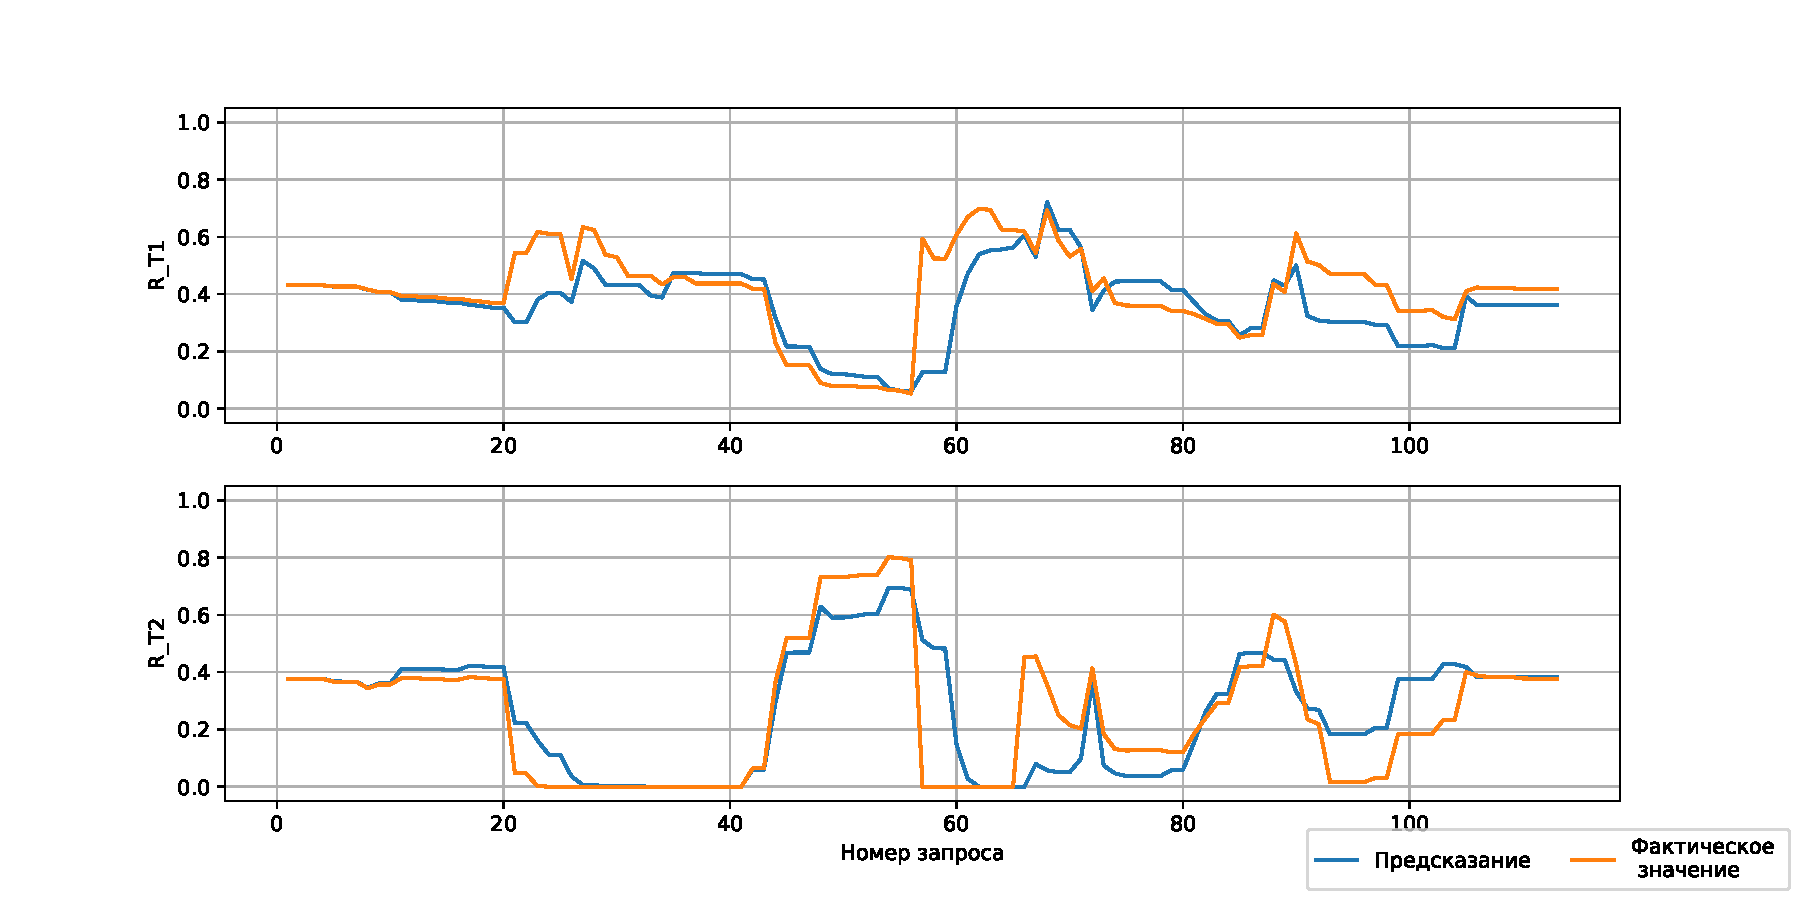
\includegraphics[width=0.95\linewidth]{images/buffer_real_113.pdf}
  \caption{Сравнение прогнозируемой и измеренной доли страниц отношений cast\_info и movie\_info в буферном кэше во время исполнения запросов бенчмарка JOB.}
  \label{fig:job-cache-validation}
\end{figure}

Полученные результаты показывают, что модель воспроизводит динамику доли резидентных страниц как в синтетических сценариях, так и при переходе к реальным отношениям и запросам. При этом значения взвешенной средней абсолютной ошибки нормированной оценки остаются близкими во всех экспериментах: для синтетических сценариев они находятся в диапазоне от 0.071 до 0.081, а при переходе к реальным данным качество оценивания не ухудшается. Результаты всех пяти экспериментов показаны в таблице \ref{tab:abs-error}.

\begin{table}[h]
\centering
\small
\begin{tblr}{
  colspec={c c},
  row{1}={font=\bfseries},
  hlines,
}
Номер эксперимента & WMAE \\
1 & 0.078 \\
2 & 0.071 \\
3 & 0.081 \\
4 & 0.061 \\
5 & 0.078 \\
\end{tblr}
\caption{Взвешенная нормализованная средняя абсолютная ошибка (WMAE) прогноза доли страниц отношений в буферном кэше.}
\label{tab:abs-error}
\end{table}

Это свидетельствует о том, что предложенная модель оценки состояния буферного кэша может использоваться как аппроксимация его текущего состояния для последующего уточнения параметров ввода-вывода стоимостной модели.

Метод адаптивной настройки параметров стоимостной модели был протестирован на аналитических бенчмарках TPC-H и JOB. На TPC-H оценивалось влияние метода на согласованность между оценочной стоимостью операторов и фактическим временем их выполнения, а также на суммарное время выполнения запросов. На JOB проводилось сравнение предложенного подхода как со стандартной стоимостной моделью, так и с методом калибровочных запросов. Результаты показали, что после применения адаптивной стоимостной модели на бенчмарке TPC-H корреляция между оценочной стоимостью узлов и фактическим временем выполнения возросла с 0.29 до 0.92, а суммарное ускорение по всему бенчмарку составило 20\%. На бенчмарке JOB предложенный метод продемонстрировал преимущество как по сравнению со стандартной стоимостной моделью, так и по сравнению с методом калибровочных запросов: суммарное время выполнения сократилось на 23.01\%, тогда как для калибровочной модели сокращение составило 18.49\%.

\underline{\textbf{Третья глава}} посвящена исследованию метода рекомендации подсказок оптимизатору на основе сопоставления планов выполнения. Известные подходы такого типа обычно опираются на специально сконструированные кодировки дерева плана или ручной выбор признаков, что требует существенной инженерной подготовки. В данной работе исследуется альтернативный подход, в котором план выполнения представляется в виде вектора, формируемого большой языковой моделью по его текстовому описанию. Под векторным представлением плана в работе понимается числовой вектор фиксированной размерности, формируемый по текстовому описанию плана, при этом близость таких векторов используется как мера сходства соответствующих планов выполнения. Это позволяет сравнивать планы выполнения и рекомендовать подсказки для новых запросов на основе ранее накопленного опыта без разработки специальной схемы представления плана и без обучения на целевой рабочей нагрузке.

Под подсказками оптимизатору понимаются управляющие указания, которые ограничивают или направляют выбор оптимизатора при построении плана выполнения запроса. Такие подсказки не изменяют результат SQL-запроса, но могут приводить к построению другого физического плана выполнения. В разных СУБД подсказки могут задавать порядок соединений таблиц, способ доступа к таблице, использование индекса или выбор физического оператора.

В данной работе рассматриваются семь бинарных управляющих параметров оптимизатора, которые делают использование соответствующих физических операторов нежелательным и тем самым направляют выбор оптимизатора. К ним относятся подсказки, связанные с выбором алгоритма соединения: \texttt{enable\_nestloop}, \texttt{enable\_hashjoin}, \texttt{enable\_mergejoin}, а также подсказки, связанные со способами доступа к данным: \texttt{enable\_seqscan}, \texttt{enable\_indexscan}, \texttt{enable\_indexonlyscan}, \texttt{enable\_bitmapscan}. Набор таких подсказок можно рассматривать как конфигурацию, задающую ограничения на пространство планов, доступное оптимизатору.

Пусть \(Q\) - входной SQL-запрос, \(P_H\) - план выполнения, построенный оптимизатором при использовании набора подсказок \(H\), а \(T(Q, P_H)\) - фактическое время выполнения соответствующего плана. Тогда задача заключается в выборе такого набора подсказок, который минимизирует время выполнения запроса:
\[
H^{*}(Q)=\arg\min_{H \in \mathcal{H}(Q)} T(Q, P_H),
\]
где \(\mathcal{H}(Q)\) обозначает множество всех допустимых конфигураций подсказок для запроса \(Q\).

На этой основе разработан метод рекомендации подсказок оптимизатору на основе сопоставления планов выполнения. Для исходного плана нового запроса в пространстве векторных представлений определяется окрестность ближайших соседей, по которой голосованием выбирается набор подсказок в качестве кандидата. После этого запрос перепланируется с выбранным кандидатом, и для исходного плана и плана-кандидата выбираются две $K$-окрестности в общем репозитории ранее наблюдавшихся планов с известными временами выполнения, после чего сравниваются средние времена выполнения в этих окрестностях. Подсказка принимается только в том случае, если среднее время выполнения в окрестности нового плана меньше. Такая двухэтапная схема уменьшает число неудачных переносов и повышает надёжность применения метода. Схема работы метода показана на рисунке~\ref{fig:plan_mapping}.

\begin{figure}[h]
  \centering
  \includegraphics[width=0.8\textwidth]{images/plan_mapping.pdf}
  \caption{Двухэтапный выбор подсказки: голосование среди $N$ ближайших
соседей планов по умолчанию для выбора кандидата, затем проверка кандидата
по двум $K$-окрестностям в общем репозитории ранее наблюдавшихся планов.}
  \label{fig:plan_mapping}
\end{figure}

Экспериментальная оценка метода рекомендации подсказок на основе сопоставления планов выполнена на наборе CEB. Полученные результаты показывают, что метод обеспечивает сокращение совокупного времени выполнения запросов: по десяти разбиениям выборки среднее ускорение составило \(19.1\%\), при этом минимальный выигрыш на отдельном разбиении составил \(8\%\), а максимальный - \(32\%\). Наибольший эффект наблюдается для наиболее медленных запросов: значение 90-го перцентиля времени выполнения снижается примерно на \(25\%\), тогда как медианное время уменьшается на \(2.1\%\). Использование только векторных представлений уже даёт положительный эффект, а добавление двухэтапной проверки согласованности дополнительно повышает качество рекомендации и уменьшает число неудачных применений подсказок. Итоговые результаты метода приведены на рисунке~\ref{fig:plan_mapping_res}: по оси абсцисс показан номер разбиения при кросс-валидации, по левой оси ординат - совокупное время выполнения запросов тестовой части для стандартного оптимизатора и предложенного алгоритма, а по правой оси ординат - относительное сокращение времени выполнения в процентах.

\begin{figure}[h]
  \centering
  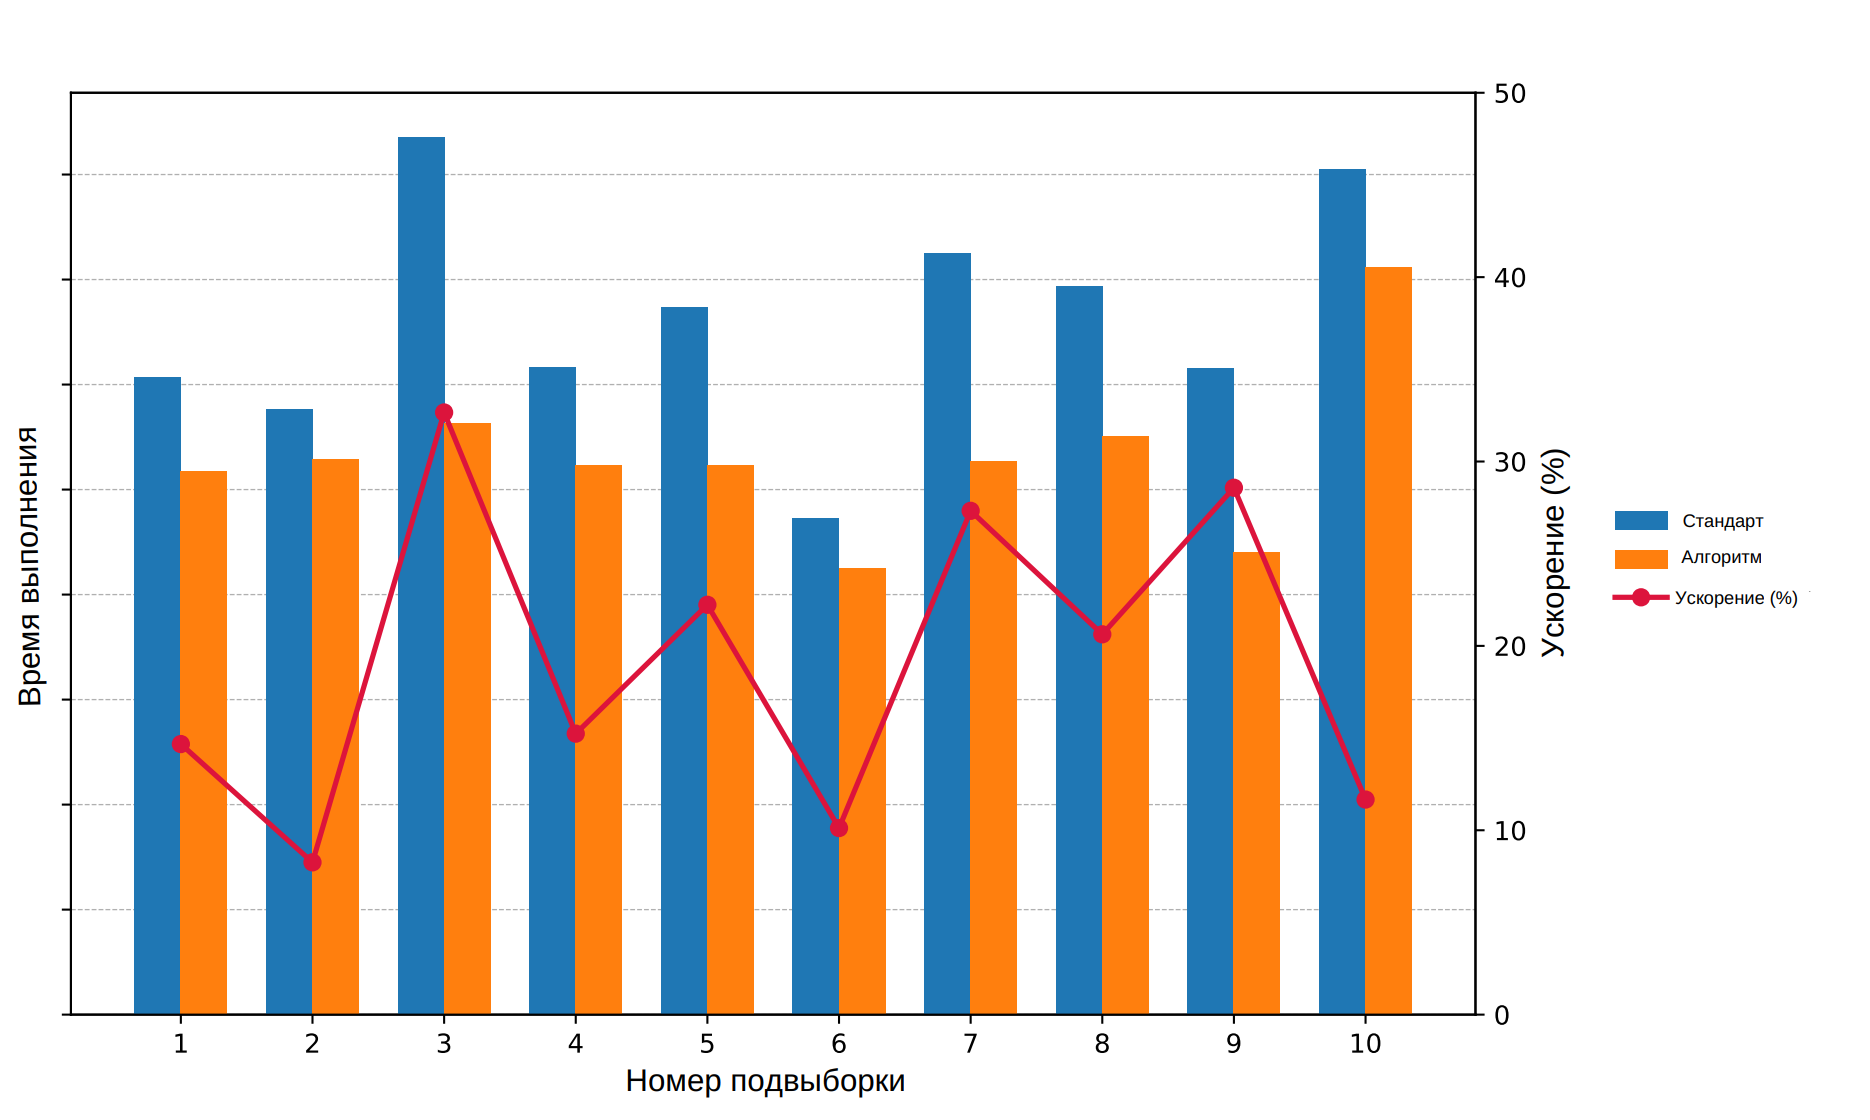
\includegraphics[width=0.8\textwidth]{images/infographic_small.png}
  \caption{Относительное изменение времени выполнения по разбиениям кросс-валидации для метода рекомендации подсказок на основе сопоставления планов.}
  \label{fig:plan_mapping_res}
\end{figure}

Для обоснования использования векторных представлений планов выполнения в задаче рекомендации подсказок в работе дополнительно рассматривается вспомогательная задача ранжирования планов по ожидаемому времени выполнения. Эта задача вводится не как самостоятельная альтернатива методу рекомендации подсказок, а как инструмент проверки того, содержат ли векторные представления планов достаточно информации для сопоставления планов по их ожидаемой эффективности. Если представления позволяют корректно восстанавливать относительный порядок планов по времени выполнения, то их можно использовать как основу для поиска похожих планов и последующей рекомендации подсказок в основной задаче главы.

Формально, для выборки запросов \(Q=\{Q_i\}_{i=1}^{N}\) и соответствующих им планов выполнения \(P=\{P_i\}_{i=1}^{N}\), для которых известно измеренное время выполнения \(T_i=T(Q_i,P_i)\), требуется построить функцию оценки
\[
s(P)\in\mathbb{R},
\]
которая по плану \(P\) возвращает скалярную величину, согласованную с истинным временем выполнения. Основное требование к такой функции задаётся в терминах относительного порядка планов:
\[
T(Q,P_a) > T(Q,P_b)\;\Rightarrow\; s(P_a) > s(P_b),
\]
по крайней мере для большинства сравниваемых пар планов. Иными словами, вспомогательная задача состоит в построении такой оценки плана, которая позволяет корректно упорядочивать планы по ожидаемой длительности выполнения.

Рассматриваются три варианта построения функции \(s(P)\): стоимостная оценка стандартного оптимизатора, модель на основе ручной структурной кодировки дерева плана, реализованная по архитектуре, предложенной в работе~\cite{10.1145/3448016.3452838}, и модель на основе векторных представлений плана, формируемых большой языковой моделью. Во втором варианте используется подход, в котором план выполнения сначала преобразуется в ручную структурную кодировку дерева плана, а затем обрабатывается свёрточной нейронной сетью по деревьям с последующей агрегацией и полносвязными слоями, предсказывающими время выполнения плана. Далее этот подход называется Bao-подобным, подчеркивая связь с известным подходом Bao~\cite{10.1145/3448016.3452838}. В предлагаемом варианте блок ручной структурной кодировки и специализированной обработки дерева заменяется использованием векторного представления плана, формируемого большой языковой моделью по его текстовому описанию.

Результаты сравнения трех подходов приведены в таблице~\ref{tab:jobceb-ranking-summary}. Видно, что при случайном разбиении выборки модель на основе векторных представлений и подход на основе кодировки планов существенно превосходят стоимостную оценку стандартного оптимизатора по качеству глобального ранжирования планов. При этом лучшие модели на основе векторных представлений не только сопоставимы с подходом Bao, но и превосходят его по рассматриваемым метрикам. Это означает, что векторные представления, формируемые большой языковой моделью, могут использоваться вместо ручной структурной кодировки плана без потери качества, а в ряде случаев и с улучшением результатов. 

\begin{table}[h]
\centering
\small
\begin{tblr}{
  width=\linewidth,
  colspec={X[l] X[l] c c},
  row{1}={font=\bfseries},
  hlines,
  vlines,
}
Схема разбиения & Модель / подход  & Попарная точность, $\mu \pm \sigma$ & Спирмен $\rho$, $\mu \pm \sigma$ \\

Случайное разбиение & Bao  & \(0.742 \pm 0.012\) & \(0.663 \pm 0.032\) \\
Случайное разбиение & \texttt{jina-code-embeddings-0.5b}  & \(0.765 \pm 0.014\) & \(0.715 \pm 0.030\) \\
Случайное разбиение & Оптимизатор  & \(0.537 \pm 0.009\) & \(0.085 \pm 0.031\) \\

Разбиение по группам & Bao & \(0.595 \pm 0.068\) & \(0.271 \pm 0.197\) \\
Разбиение по группам & \texttt{jina-code-embeddings-0.5b}  & \(0.597 \pm 0.087\) & \(0.283 \pm 0.248\) \\
Разбиение по группам & Оптимизатор  & \(0.614 \pm 0.079\) & \(0.316 \pm 0.222\) \\
\end{tblr}
\caption{Метрики ранжирования на наборе запросов CEB при случайном разбиении выборки и при разбиении по группам.}
\label{tab:jobceb-ranking-summary}
\end{table}

При разбиении данных по группам качество всех обучаемых моделей заметно снижается, что указывает на трудность переноса на ранее не наблюдавшиеся шаблоны запросов. В то же время для стандартного оптимизатора корреляция возрастает, что согласуется с тем, что его стоимостная оценка лучше отражает относительный порядок планов внутри структурно однородных групп, чем между различными шаблонами.

В \underline{\textbf{четвёртой главе}}  приведено описание агентного метода итеративного поиска подсказок оптимизатору при ограниченном бюджете пробных запусков. Под бюджетом пробных запусков понимается максимальное число пробных запусков запроса с различными конфигурациями подсказок, которое допускается потратить на поиск более эффективного плана. В отличие от главы 3, где используется рекомендация подсказок для нового запроса на основе ранее накопленного опыта, здесь задача формулируется как последовательный процесс выбора действий в замкнутом контуре обратной связи с СУБД. Для её решения разработан агентный метод, в котором большая языковая модель используется как компонент пошагового выбора очередного действия на основе текущего состояния поиска.

Вводится граф состояний подсказок, который строится отдельно для каждого запроса и описывает пространство допустимых переходов между конфигурациями подсказок оптимизатору. 
Для запроса \(q\) формируется ориентированный граф \(G_q=(V_q,E_q)\), где корневая вершина соответствует базовому выполнению без подсказок, каждая вершина хранит текущий набор подсказок, полученный план и измеренное время исполнения, а каждое ребро соответствует применению одной новой подсказки. 
Один граф задаёт все рассматриваемые траектории поиска для одного запроса. 
На этой основе формируется диалоговый набор данных, в котором каждой точке поиска соответствует контекст, включающий текущее состояние, историю предыдущих запусков и наблюдённую реакцию СУБД. На рисунке \ref{fig:llm_dataset} показан упрощённый пример графа состояний для одного запроса.

\begin{figure}[h]
	\centering
	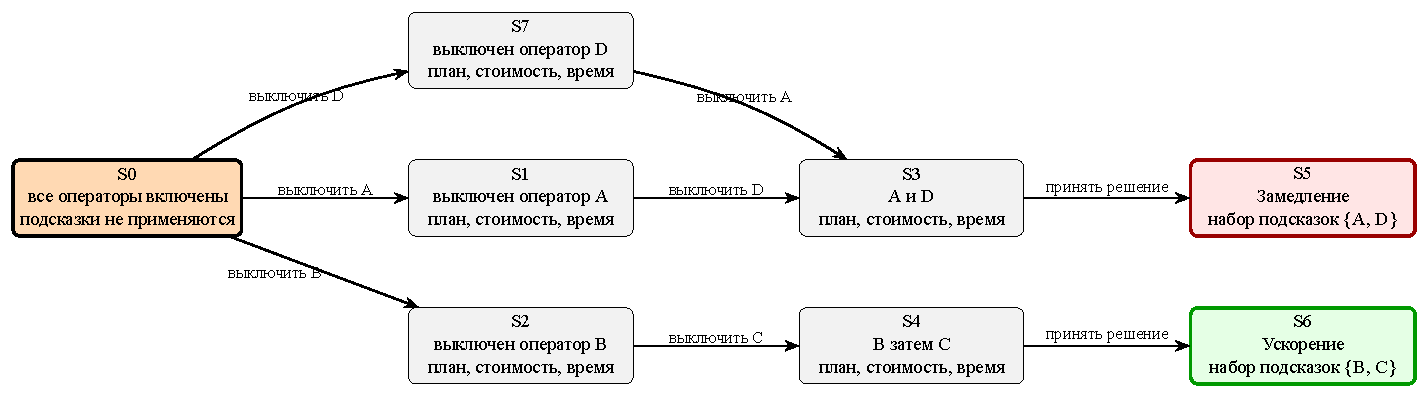
\includegraphics[width=1\textwidth]{images/llm_dataset.pdf}
	\caption{Пример графа состояний подсказок для одного запроса.}
	\label{fig:llm_dataset}
\end{figure}

Формально, пусть \(H\) обозначает множество доступных подсказок, а состояние поиска на шаге \(t\) соответствует вершине \(v_t \in V_q\), то есть \(s_t \equiv v_t\). Тогда действие агента \(a_t \in H\) соответствует выбору одного ребра \((v_t,v_{t+1}) \in E_q\), а наблюдение \(o_t\) задаётся результатом пробного запуска в вершине \(v_{t+1}\), включая полученный план и измеренное время выполнения. Процесс поиска описывается последовательностью состояний, действий и наблюдений
\[
s_{t+1}=\mathcal{T}(s_t,a_t,o_t), \qquad t=1,\dots,T,\qquad T\leq B,
\]
где \(B\) --- максимально допустимое число пробных запусков, а \(T\) --- фактическое число выполненных шагов. Иными словами, агент должен выбрать путь в графе состояний длины не более \(B\), который приводит к наилучшей конфигурации подсказок. Цель состоит в том, чтобы при ограничении на бюджет \(B\) найти такую последовательность действий, которая минимизирует время выполнения запроса после применения итогового набора подсказок. Архитектура агентной системы представлена на рисунке \ref{fig:design_dialogllm}.

\begin{figure}[htbp]
  \centering
  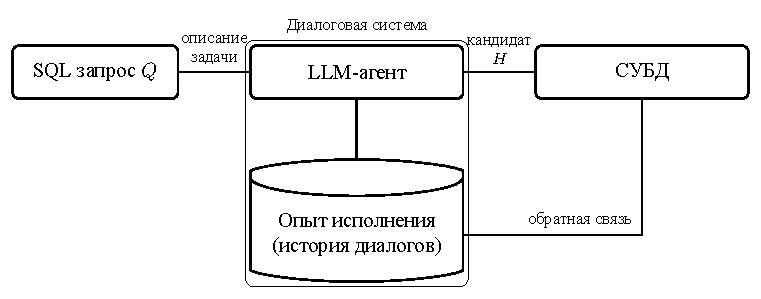
\includegraphics[width=.85\linewidth]{images/dialog_arch.pdf}
  \caption{Архитектура итеративной системы поиска подсказок оптимизатору.}
  \label{fig:design_dialogllm}
\end{figure}

Для экспериментальной оценки предложенного подхода в главе рассматриваются несколько групп методов. В качестве методов сравнения используются базовые стратегии перебора на графе состояний подсказок: случайный поиск, случайный поиск с безопасным принятием и жадный поэтапный перебор. Также рассматривается адаптированный вариант Bao как обучаемый метод выбора подсказок оптимизатору в постановке ограниченного бюджета пробных запусков. В качестве предлагаемых методов исследуются два варианта агентной реализации на основе большой языковой модели: контекстный агент без дообучения и дообученный агент, обученный на корпусе целевых траекторий поиска, извлечённых из графов состояний подсказок. Это позволяет сопоставить предлагаемые агентные методы как с простыми стратегиями перебора, так и с обучаемым подходом к выбору подсказок оптимизатору.

Экспериментально установлено, что при ограниченном бюджете пробных запусков агентные методы обеспечивают наибольшее ускорение на ранних этапах поиска. Уже на первом шаге дообученный агент достигает \(58.0\%\) ускорения, контекстный агент --- \(52.1\%\), тогда как адаптированный Bao показывает \(41.8\%\), а базовые стратегии перебора --- около \(32\%\). К пятому шагу дообученный агент сохраняет лидерство с ускорением \(67.3\%\). Это показывает, что использование большой языковой модели позволяет быстрее находить эффективные конфигурации подсказок при малом бюджете пробных запусков. Результаты показаны на рисунке~\ref{fig:boost_llm}.

Как показано на рисунке~\ref{fig:methods_cost_agent}, методы существенно различаются по стоимости одного пробного запуска. На интервале малых бюджетов, представляющем основной практический интерес для рассматриваемой постановки, наименьшую относительную стоимость пробного запуска показывает дообученный агент. Контекстный агент и адаптированный Bao также демонстрируют устойчивое поведение, тогда как переборные стратегии оказываются менее выгодными по затратам на одну попытку.

Рост стоимости случайного поиска по пути к шагу \(K=7\) объясняется тем, что данный алгоритм последовательно накапливает отключения операторов и не использует механизм безопасного принятия. К седьмому шагу все семь рассматриваемых управляющих параметров переведены в состояние \texttt{off}. При такой конфигурации подсказок оптимизатор по возможности избегает соответствующих операторов, а при невозможности построить корректный план без них использует их с существенно увеличенной оценочной стоимостью. В результате предпочтения оптимизатора сильно искажаются, и пробные запуски могут становиться дорогими. После завершения пути алгоритм начинает новый путь из начального состояния, поэтому на шаге \(K=8\) относительная стоимость снижается.

Тем самым показано, что агентные методы не только обеспечивают более высокое качество ранних решений, но и позволяют получать это преимущество при меньших относительных затратах на отдельный шаг оптимизации. 

\begin{figure}[h]
  \centering
  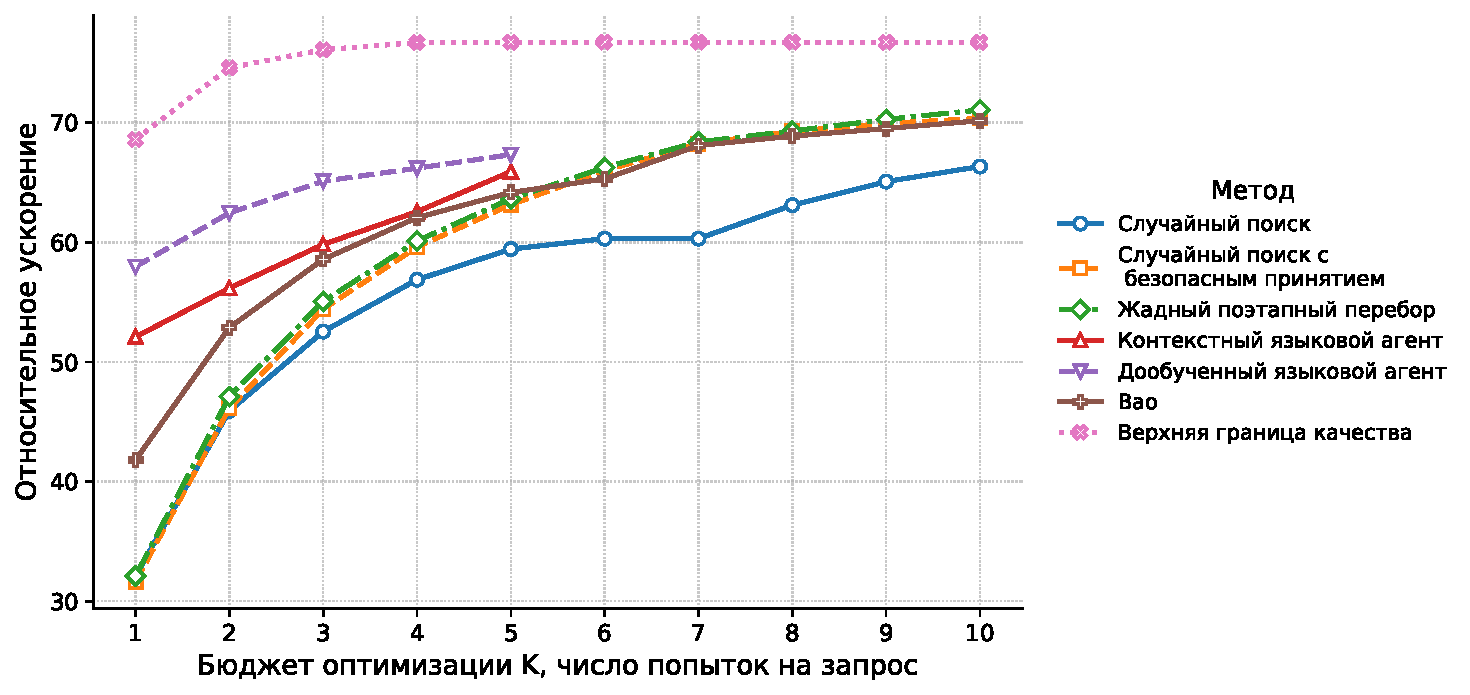
\includegraphics[width=.85\linewidth]{images/boost_vs_budget_7arm_ru.pdf}
  \caption{Сравнение методов по максимальному достигнутому ускорению при ограниченном бюджете пробных запусков.}
  \label{fig:boost_llm}
\end{figure}

\begin{figure}[h]
  \centering
  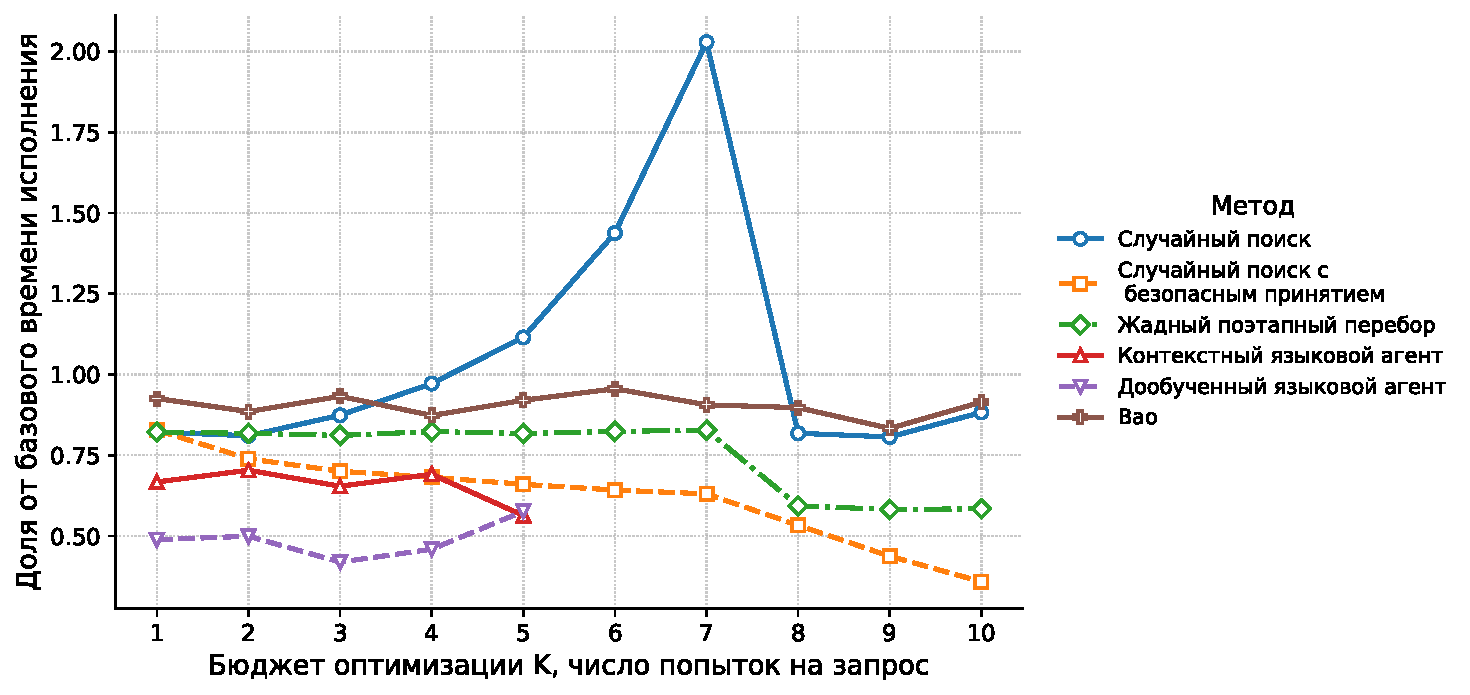
\includegraphics[width=.85\linewidth]{images/step_budget.pdf}
    \caption{Относительная стоимость одного шага оптимизации в долях от стандартного времени выполнения.}
  \label{fig:methods_cost_agent}
\end{figure}

\FloatBarrier
\pdfbookmark{Заключение}{conclusion}                                  % Закладка pdf
В \underline{\textbf{заключении}} приведены основные результаты исследования.

\begin{itemize}
    \item Разработаны метод адаптивной настройки параметров стоимостной модели оптимизатора по телеметрии фактически выполняемых запросов, метод рекомендации подсказок оптимизатору на основе сопоставления планов выполнения и агентный метод итеративного поиска подсказок оптимизатору при ограниченном бюджете пробных запусков.

    \item На аналитических бенчмарках TPC-H, JOB и CEB установлено, что предложенные методы обеспечивают повышение качества выбора планов выполнения, сокращение совокупного времени выполнения запросов и преимущество по сравнению со стандартным оптимизатором и сравниваемыми подходами. Показано, что векторные представления планов, формируемые большой языковой моделью, пригодны для рекомендации подсказок на основе ранее накопленного опыта, а агентный метод особенно эффективен на ранних шагах итеративного поиска.

    \item Показано, что результаты работы могут применяться для практического ускорения аналитических запросов, автоматизации настройки оптимизатора и совершенствования внутренних механизмов планирования в реляционных системах управления базами данных.
\end{itemize}



%% Переработанное заключение без перечисления экспериментальных показателей.
% Заголовок \chapter*{Заключение} при необходимости добавляется в основном файле.

В работе решена научно-прикладная задача повышения эффективности оптимизации SQL-запросов за счёт разработки методов, дополняющих штатный стоимостный оптимизатор без его полной замены. Предложены три взаимодополняющих направления: адаптивная настройка параметров стоимостной модели по телеметрии рабочей нагрузки, рекомендация подсказок оптимизатору на основе сопоставления планов выполнения в пространстве векторных представлений и агентный итеративный поиск подсказок при ограниченном бюджете пробных запусков. Поставленная цель достигнута, сформулированные задачи выполнены.

Предложенные методы предназначены для различных практических ситуаций и не должны рассматриваться как обязательные последовательные этапы единого алгоритма. Метод адаптивной настройки воздействует на параметры стоимостной модели, метод рекомендации использует ранее накопленный опыт для быстрого выбора подсказок в онлайн-режиме, а агентный метод решает отдельную задачу оффлайн-поиска новой конфигурации. Совместное применение этих методов в работе экспериментально не исследовалось, поэтому при их комбинировании необходимо отдельно оценивать итоговый план: влияние изменения параметров стоимостной модели и подсказок оптимизатору может быть неаддитивным.

Практическое применение метода адаптивной настройки стоимостной модели целесообразно в случаях, когда оценки кардинальности в целом достаточно корректны, однако штатные параметры стоимости не отражают фактические характеристики аппаратной среды, состояние буферного кэша или особенности рабочей нагрузки. Метод не предназначен для исправления ошибок оценки кардинальности. Поэтому его применению должна предшествовать диагностика причины неэффективного выбора плана. Если основная ошибка возникает на уровне кардинальностей, корректировка стоимостных коэффициентов не устраняет первопричину; если же рассогласование связано со стоимостью ввода-вывода или вычислительных операций, адаптивная настройка может использоваться для уточнения штатной модели.

Состояние буферного кэша в предложенном методе оценивается агрегированно на уровне отношений, без отслеживания отдельных страниц. Это снижает требования к памяти и вычислительные накладные расходы, но требует накопления достаточного числа наблюдений, поэтому результаты начального периода работы следует интерпретировать осторожно. При практическом внедрении необходимо также учитывать взаимодействие динамической оценки резидентности со штатными механизмами СУБД, в частности с параметрами, уже учитывающими предполагаемое кэширование данных. Отдельной задачей дальнейшего развития является исключение возможного частичного двойного учёта эффекта буферного кэша и более тесная интеграция динамической оценки резидентности в штатную стоимостную модель.

Метод рекомендации подсказок на основе сопоставления планов наиболее естественно применять для стационарных или частично повторяющихся аналитических нагрузок, где уже накоплена история выполнения запросов и для нового запроса можно найти структурно близкие ранее наблюдавшиеся планы. Близость векторных представлений используется только для формирования конфигурации-кандидата и не является достаточным основанием для её безусловного применения. После повторного планирования выполняется дополнительная проверка согласованности по накопленному репозиторию. Если подходящего локального опыта недостаточно либо кандидат не проходит проверку, онлайн-метод должен отказаться от рекомендации и сохранить штатную конфигурацию оптимизатора. Такой отказ является нормальным результатом работы метода, а оффлайн-поиск не запускается автоматически как его внутренняя ветвь.

При использовании онлайн-метода следует учитывать стоимость дополнительного планирования, построения векторных представлений и поиска ближайших соседей. Поэтому он прежде всего ориентирован на аналитические запросы, для которых ожидаемый выигрыш от улучшенного плана превышает стоимость этапа рекомендации. При росте репозитория накопленного опыта целесообразно использовать индексированные методы приближённого поиска ближайших соседей вместо полного линейного перебора. Перенос метода на СУБД с существенно иной системой физических операторов или иным представлением планов требует отдельной проверки пригодности используемых векторных представлений.

Агентный метод итеративного поиска подсказок предназначен для оффлайн-оптимизации запросов, когда допустим заранее заданный бюджет пробных запусков. Он может применяться при отсутствии достаточного накопленного опыта, при невозможности сформировать надёжную онлайн-рекомендацию или как самостоятельный механизм дополнительной оптимизации длительно выполняющихся запросов. Языковая модель в этом случае используется как компонент принятия решений, который анализирует текущее состояние поиска, результаты предыдущих попыток и выбирает следующее действие. Метод следует рассматривать как эвристический механизм направленного поиска, ориентированный на рациональное использование ограниченного бюджета, а не как алгоритм, гарантирующий нахождение глобально оптимальной конфигурации.

Практическая ценность агентного подхода возрастает по мере увеличения пространства допустимых конфигураций, когда полный перебор становится слишком дорогим. Вместе с тем при реальном внедрении необходимо учитывать полную стоимость оффлайн-оптимизации, включая не только пробные выполнения запросов, но и время обращения к языковой модели. Применение агентного поиска оправдано прежде всего для длительных или многократно повторяющихся запросов, для которых затраты предварительной оптимизации могут быть компенсированы последующими выполнениями.

Для практического выбора метода администратором базы данных можно использовать следующую схему:
\begin{enumerate}
    \item Если проблема связана преимущественно с несоответствием параметров стоимостной модели фактической среде выполнения при достаточно корректных оценках кардинальности, целесообразно применять адаптивную настройку стоимостной модели.
    \item Если для текущего запроса имеется накопленная история структурно близких планов с известными эффективными конфигурациями подсказок, целесообразно использовать онлайн-метод рекомендации на основе сопоставления планов.
    \item Если близкие аналоги отсутствуют либо найденная рекомендация не проходит проверку, для длительного запроса может быть отдельно запущен агентный оффлайн-поиск с заранее установленным бюджетом пробных запусков.
    \item Результаты оффлайн-оптимизации целесообразно сохранять в репозитории накопленного опыта и использовать при последующих онлайн-рекомендациях, постепенно расширяя область запросов, для которых дорогостоящий поиск не требуется.
    \item При совместном применении нескольких предложенных методов итоговый план необходимо валидировать отдельно, поскольку экспериментальных оснований считать их эффекты независимыми или аддитивными в работе не получено.
\end{enumerate}

Для инженеров СУБД полученные результаты представляют интерес как основа для совершенствования внутренних механизмов планирования. Сопоставление исходных и улучшенных планов позволяет выявлять случаи, в которых штатная стоимостная модель, ограничения пространства поиска или выбор физических операторов приводят к менее эффективному решению. Предложенные методы сохраняют существующий оптимизатор в качестве основного механизма построения планов и дополняют его средствами адаптации, переноса накопленного опыта и направленного поиска.


\medskip
\noindent
\textbf{Перспективы дальнейшего развития направления.}
Дальнейшее развитие работы связано как с углублением отдельных предложенных методов, так и с исследованием их совместного применения в более общей системе поддержки решений по оптимизации запросов.

Для метода адаптивной настройки стоимостной модели перспективным направлением является более тесная интеграция динамической оценки резидентности отношений со штатными механизмами СУБД. В частности, представляет интерес использование наблюдаемого состояния буферного кэша непосредственно при оценке ожидаемого числа обращений к памяти и диску, что позволит уменьшить риск частичного двойного учёта эффекта кэширования. Отдельного исследования требуют устойчивость метода при длительной конкурентной нагрузке, сценарии с операциями записи, полные накладные расходы на сбор телеметрии и минимальный объём наблюдений, необходимый для выхода модели в устойчивый режим. Перспективной является также разработка диагностического механизма, позволяющего различать ошибки стоимостной модели и ошибки оценки кардинальности и тем самым выбирать корректный способ воздействия на оптимизатор.

Для метода рекомендации подсказок на основе сопоставления планов основным направлением является повышение качества переноса на ранее не наблюдавшиеся шаблоны запросов. Для этого могут исследоваться доменная адаптация моделей векторных представлений, дополнительное обучение на планах выполнения, объединение текстовых и структурных признаков и гибридные метрики близости. Практически важны также разработка явного критерия уверенности рекомендации, масштабирование репозитория с использованием индексных методов приближённого поиска ближайших соседей и учёт устаревания накопленного опыта при изменении данных, конфигурации СУБД и аппаратной платформы. Отдельного изучения требует перенос метода на СУБД с иной системой физических операторов и другим представлением планов.

Для агентного метода наиболее существенным продолжением является переход к более крупным пространствам действий, в которых подсказки задаются не только глобально для классов операторов, но и локально для отдельных соединений, отношений, индексов и способов доступа. В такой постановке полный перебор становится практически невозможным, а направленный поиск при ограниченном бюджете приобретает ещё большее значение. Дополнительным направлением является развитие политики агента за счёт использования накопленных в эксплуатации успешных и неуспешных траекторий для периодического дообучения и формирования более информативного контекста.

Отдельным направлением дальнейшей работы является экспериментальная проверка совместного применения методов глав~2--4. Наиболее общей постановкой здесь является создание диагностического механизма, который по характеристикам запроса, состоянию СУБД и накопленной истории определяет причину неэффективного планирования и выбирает подходящее действие: корректировку стоимостной модели, онлайн-перенос конфигурации по аналогии, агентный оффлайн-поиск либо сохранение штатного решения. Такая система должна учитывать возможное неаддитивное взаимодействие методов и отдельно проверять качество итогового плана после каждого изменения.

Таким образом, диссертационная работа показывает возможность повышения качества планирования аналитических SQL-запросов без полной замены существующего оптимизатора. Предложенные методы могут использоваться как самостоятельные средства в различных диагностических ситуациях и как элементы более общей системы управления качеством планирования. Выбор конкретного метода должен определяться причиной неэффективного планирования, характером рабочей нагрузки, наличием накопленного опыта и допустимой стоимостью дополнительной оптимизации.


\pdfbookmark{Литература}{bibliography}                                % Закладка pdf
%При использовании пакета \verb!biblatex! список публикаций автора по теме
%диссертации формируется в разделе <<\publications>>\ файла
%\verb!common/characteristic.tex!  при помощи команды \verb!\nocite!

\ifdefmacro{\microtypesetup}{\microtypesetup{protrusion=false}}{} % не рекомендуется применять пакет микротипографики к автоматически генерируемому списку литературы
\urlstyle{rm}                               % ссылки URL обычным шрифтом
\ifnumequal{\value{bibliosel}}{0}{% Встроенная реализация с загрузкой файла через движок bibtex8
    \renewcommand{\bibname}{\large \bibtitleauthor}
    \nocite{*}
    \insertbiblioauthor           % Подключаем Bib-базы
    %\insertbiblioexternal   % !!! bibtex не умеет работать с несколькими библиографиями !!!
}{% Реализация пакетом biblatex через движок biber
    % Цитирования.
    %  * Порядок перечисления определяет порядок в библиографии (только внутри подраздела, если `\insertbiblioauthorgrouped`).
    %  * Если не соблюдать порядок "как для \printbibliography", нумерация в `\insertbiblioauthor` будет кривой.
    %  * Если цитировать каждый источник отдельной командой --- найти некоторые ошибки будет проще.
    %
    %% authorvak

    \ifnumgreater{\value{usefootcite}}{0}{
        \begin{refcontext}[labelprefix={}]
            \ifnum \value{bibgrouped}>0
                \insertbiblioauthorgrouped    % Вывод всех работ автора, сгруппированных по источникам
            \else
                \insertbiblioauthor      % Вывод всех работ автора
            \fi
        \end{refcontext}
    }{
        \ifnum \totvalue{citeexternal}>0
            \begin{refcontext}[labelprefix=A]
                \ifnum \value{bibgrouped}>0
                    \insertbiblioauthorgrouped    % Вывод всех работ автора, сгруппированных по источникам
                \else
                    \insertbiblioauthor      % Вывод всех работ автора
                \fi
            \end{refcontext}
        \else
            \ifnum \value{bibgrouped}>0
                \insertbiblioauthorgrouped    % Вывод всех работ автора, сгруппированных по источникам
            \else
                \insertbiblioauthor      % Вывод всех работ автора
            \fi
        \fi
        %  \insertbiblioauthorimportant  % Вывод наиболее значимых работ автора (определяется в файле characteristic во второй section)
        \begin{refcontext}[labelprefix={}]
            \insertbiblioexternal            % Вывод списка литературы, на которую ссылались в тексте автореферата
        \end{refcontext}
        % Невидимый библиографический список для подсчёта количества внешних публикаций
        % Используется, чтобы убрать приставку "А" у работ автора, если в автореферате нет
        % цитирований внешних источников.
        \printbibliography[heading=nobibheading, section=0, env=countexternal, keyword=biblioexternal, resetnumbers=true]%
    }
}
\ifdefmacro{\microtypesetup}{\microtypesetup{protrusion=true}}{}
\urlstyle{tt}                               % возвращаем установки шрифта ссылок URL
